\documentclass{article}
%\documentclass[a4paper,12pt,twoside]{book}
\usepackage{amsmath}
\usepackage{cite}
%\usepackage{tikz}
\usepackage{bm}
\usepackage{tikz,tkz-tab}
\usepackage{amsfonts}%
\usepackage{amssymb}%
\usepackage{hyperref}
\usepackage{mathtools}
%\usepackage{subcaption}
\usepackage{color}
\usepackage{multicol}
\usepackage{setspace}
\usepackage{empheq}
\usepackage{bbm, dsfont}
\usepackage{dsfont}
\usepackage{mathtools}
\usepackage[left=1.8cm, right=1.8cm, top=1.5cm]{geometry}
\usepackage{enumitem} 
\usepackage[bottom]{footmisc}
\usetikzlibrary{arrows}
\usepackage{lscape}
\usepackage{tcolorbox}
\usepackage{caption}
%\usepackage{graphicx}
\usepackage{subfig}
\usepackage{multirow}
\usepackage{cite}
\usepackage{lscape}
\usepackage{makecell}
\usetikzlibrary{shapes,snakes}
\renewcommand{\labelitemi}{$\bullet$}
\renewcommand{\labelitemii}{$\diamond$}

\usepackage{titlesec}
\usepackage[font=footnotesize,labelfont=bf]{caption}

\setcounter{secnumdepth}{4}

\titleformat{\paragraph}
{\normalfont\normalsize\bfseries}{\theparagraph}{1em}{}
\titlespacing*{\paragraph}
{0pt}{3.25ex plus 1ex minus .2ex}{1.5ex plus .2ex}


\newtheorem{definition}{Definition}

\usetikzlibrary{positioning}
\tikzset{main node/.style={circle,draw,minimum size=0.5cm,inner sep=0pt},
            }

%-------------------------------------------
\newtheorem{example}{Example}
\newtheorem{theorem}{Theorem}
\newtheorem{acknowledgement}[theorem]{Acknowledgement}
\newtheorem{algorithm}[theorem]{Algorithm}
\newtheorem{axiom}[theorem]{Axiom}
\newtheorem{case}[theorem]{Case}
\newtheorem{claim}{Claim}
\newtheorem{conclusion}[theorem]{Conclusion}
\newtheorem{condition}[theorem]{Condition}
\newtheorem{conjecture}[theorem]{Conjecture}
\newtheorem{corollary}{Corollary}
\newtheorem{criterion}[theorem]{Criterion}
\newtheorem{assumption}{Assumption}
\newtheorem{exercise}[theorem]{Exercise}
\newtheorem{lemma}{Lemma}
\newtheorem{observation}{Observation}
\newtheorem{notation}[theorem]{Notation}
\newtheorem{problem}[theorem]{Problem}
\newtheorem{proposition}{Proposition}
\newtheorem{remark}{Remark}
\newtheorem{solution}[theorem]{Solution}
\newtheorem{summary}[theorem]{Summary}
\newenvironment{proof}[1][Proof]{\textbf{#1.} }{\ \rule{0.5em}{0.5em}}




\begin{document}

\title{Twi Clim}
%\date{}
\author{Shaden Shabayek\footnote{Post-doctoral researcher at the m\'{e}dialab SciencesPo. Contact: shaden.shabayek@sciencespo.fr}}
\maketitle{}

\onehalfspace

\section{introduction}

\section{Methods \& Materials}

We build a dataset of Twitter accounts, which we categorize as promoting science (a priori high reliability) or activism either to promote or oppose climate actions (of unknown a priori reliability). The three groups are: climate “Scientists”, climate “Activists” and climate “Delayers”. We populate these three groups following the process outlined in Figure xx and we provide details below.  

\subsection{Construction of “Elite” groups: Scientists, Activists \& Delayers}

First, we populate the group of climate “Scientists” by taking the 3180 Twitter accounts (as of April 2022) who belong to the list “Scientists who do climate” created by Dr Katharine Hayhoe. Second, we build a group of climate “Delayers” by scraping the Twitter handles which appear on the profiles of individuals and organizations in the “Desmog climate disinformation database”. This results in 521 individuals and 270 organizations with a dedicated page containing background information, stance on climate change and social media accounts when they exist. Among this set of individuals and organizations, only 325 had an existing and active Twitter account. Moreover, 14 accounts were suspended on Twitter for violating Twitter rules. We recovered the users metrics (number of followers, number of tweets, creation date of the account, biography description, etc.) of all the active accounts from the Twitter API V2 using the users/by/username endpoint. Then we applied a followers-based influence measure by only keeping in our initial sample Twitter accounts with over 10k followers. This threshold corresponds respectively to the 96\% and 59\% cut-off of followers count for the climate “Scientists” and climate “Delayers” Twitter accounts. This gives 135 Twitter climate “Scientists” and 66 Twitter climate “Delayers”, which are used as seed groups. Furthermore, we follow an event-based approach and build a control group by searching for Tweets containing the hashtag  \#COP26 during COP26 from October 31 to November 12, 2021. Doing so we obtain 1.3 million tweets (excluding retweets) created by 400k unique Twitter users. We keep Twitter users with over 10k followers (90\% cut-off of followers count) and filter out those who have the following keywords in their Twitter account description: climate activist, environmental activist, environmentalist. This results in 105 Twitter climate “Activists”. 
Finally, we define an Elite Twitter account as an account such that the number of followers is over 10k in reference to the 90\% cut-off followers count for the sample of users who tweeted COP26 during COP26. We remove from the control group by hashtag selection users who come up and who already belong to the groups climate “Scientists” and climate “Delayer”.

\begin{figure}
	\centering
	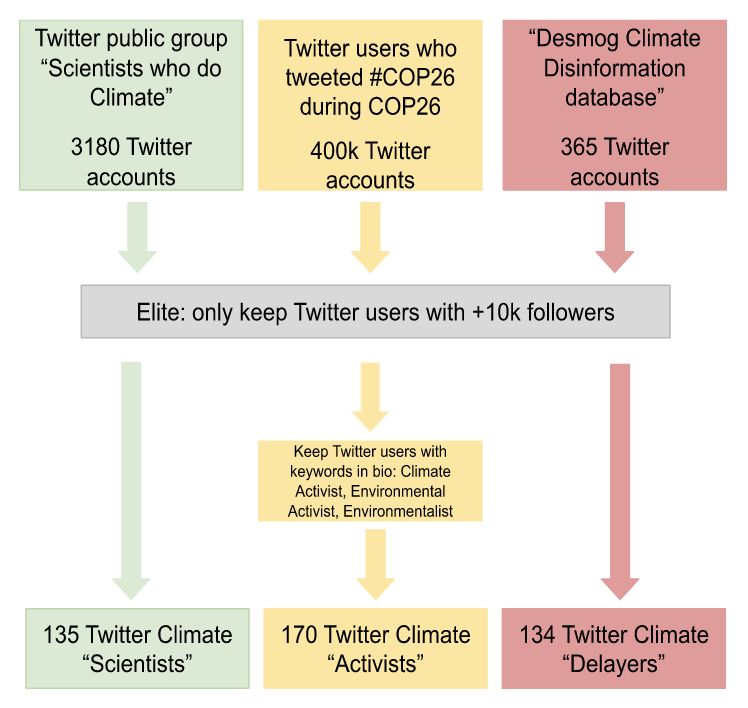
\includegraphics[scale=0.8]{./img/actors.png}
	\caption{process of initial “Elite” Twitter accounts selection}
	\label{actors}
\end{figure}
\subsection{Data collection}

We use the historical search endpoint ‘api.twitter.com/2/tweets/search/all’ available for the academic track of the Twitter API v2, in order to collect the Tweets of all users in the three seed groups over the last 6 month of 2021. We collect the content of tweets, the engagement metrics (likes, retweets, replies count), hashtags if they exist, expanded URL links within tweets. Notice that links included within tweets appear in a shortened format and for some tweets the fields returned by the API are enriched to include the fully expanded URL (‘unwound\_url’ field). When this field does not exist we use during collection from the minet python library the ‘multithreaded\_resolve’ function in order to expand the URL. We also use the ‘get\_domain\_name’ function from the “ural” python library to obtain for each URL the domain name. The collection runs from 19/07/2022 to 21/07/2022 and results in around one million Tweets.

\subsection{Domain names factual check ratings} 

We compile a dataset of domain names ratings based on the factual check ratings provided by the website Media Bias Fact Check. This website aggregates multiple fact-checks and assigns a rating (very-low, low, mixed, high, very-high, mostly-factual) to domain names. We combine two approaches to build this dataset. 

First we use the Iffy public spreadsheet to get an initial list of domain names ratings. This dataset aggregates a list of websites rated as of low or very-low credibility, based on data pulled from the Media Bias Fact Check (MBFC) website. 
Second, since the iffy spreadsheet only includes domain names with very-low and low ratings we designed a semi-automated process to obtain domain name ratings that were not limited to low credibility. From the set of collected Tweets, we identified 374 618 Tweets containing URL links. As a first step, we obtained the domain names of these URLs, which amounted to 22 537 unique cited domain names. Then we sorted the domain names by repetition in ascending order. For example, the domain name “theguardian.com” is the top cited domain name and it appeared 22 157 times within Tweets, followed by “nytimes.com” which appeared 8 030 times within Tweets in our corpus. As a second step, we manually looked up on the Media Bias Factual Check for the ratings of 500 domain names with highest occurrence. 

\section{Results}

\section{Dataset description}
By selecting two groups with a priori different levels of “credibility”  (Scientists and Delayers) along with a control group (Activists), we are set out to try and point out differences in terms of online posting behaviors and characteristics. 
A few patterns emerge from preliminary analysis of the Twitter corpus of one million Tweets by climate “Scientists”, “Activists” and “Delayers”. Almost half of the corpus consists of Retweets and only 20.7\% correspond to “raw” Tweets with created content by a given user (see Figure 2). The three groups are almost of the same order of magnitude (see Figure 1). Yet nearly half of the Tweets correspond to the activity of users within the group climate “Activists” (see Figure 3), who also have a retweet level which is higher than their usage of Replies, Quotes and Raw Tweet creation (see Figure 6 panel b). Similarly, when looking at the Tweets including at least one Hashtag (see Figure 4), almost 58\% of these Tweets are posted by climate “Activists” and only 17\% by climate “Delayers”. This result suggests that the Tweeting behavior is different across “a priori” different groups and that investigating an online phenomena through hashtag analysis might over-estimate the presence of actors who vigorously use hashtags. Similarly when looking at Tweets containing at least one link (see Figure 5), we find that climate “Delayers” and climate activists are responsible for an equal share of 39\% of these Tweets against only 22\% posted by climate “Scientists”. Again, the three groups seem to exhibit differences in terms of volume of “source” citations and focusing an investigation merely on the analysis of links can under-estimate the participation of a group to the online discourse on climate. 

\begin{figure}[ht] \label{ fig7} 
  \begin{minipage}[b]{0.4\linewidth}
  \centering
    \includegraphics[width=.6\linewidth]{../figures/share_type_tweet.jpg} 
    \caption{share of Tweets by type of Tweet in the corpus of 1 million Tweets} 
  \end{minipage} 
  \begin{minipage}[b]{0.4\linewidth}
  \centering
    \includegraphics[width=.6\linewidth]{../figures/share_tweet_by_group.jpg} 
    \caption{share of Tweets (including retweets, quotes, replies) by group in the corpus of 1 million Tweets.} 
  \end{minipage} 
  \begin{minipage}[b]{0.4\linewidth}
  \centering
    \includegraphics[width=.6\linewidth]{../figures/share_hashtags_by_group.jpg} 
    \caption{share of Tweets including at least one hashtag by group, corresponding to 272 666 unique Tweets (including retweets, quotes, replies) and 90 475 unique hashtags.} 
  \end{minipage}
  \hfill
  \hfill
  \begin{minipage}[b]{0.4\linewidth}
  \centering
    \includegraphics[width=.6\linewidth]{../figures/share_url_clim.jpg} 
    \caption{share of URLs contained within Tweets by group out of a total of 386 070 URLs in the corpus, corresponding to 374 425 unique Tweets (including retweets, quotes, replies) and 22 228 unique cited domain names.} 
  \end{minipage} 
\end{figure}

%%

\begin{figure}[ht] \label{ fig7} 
  \begin{minipage}[b]{0.4\linewidth}
  \centering
    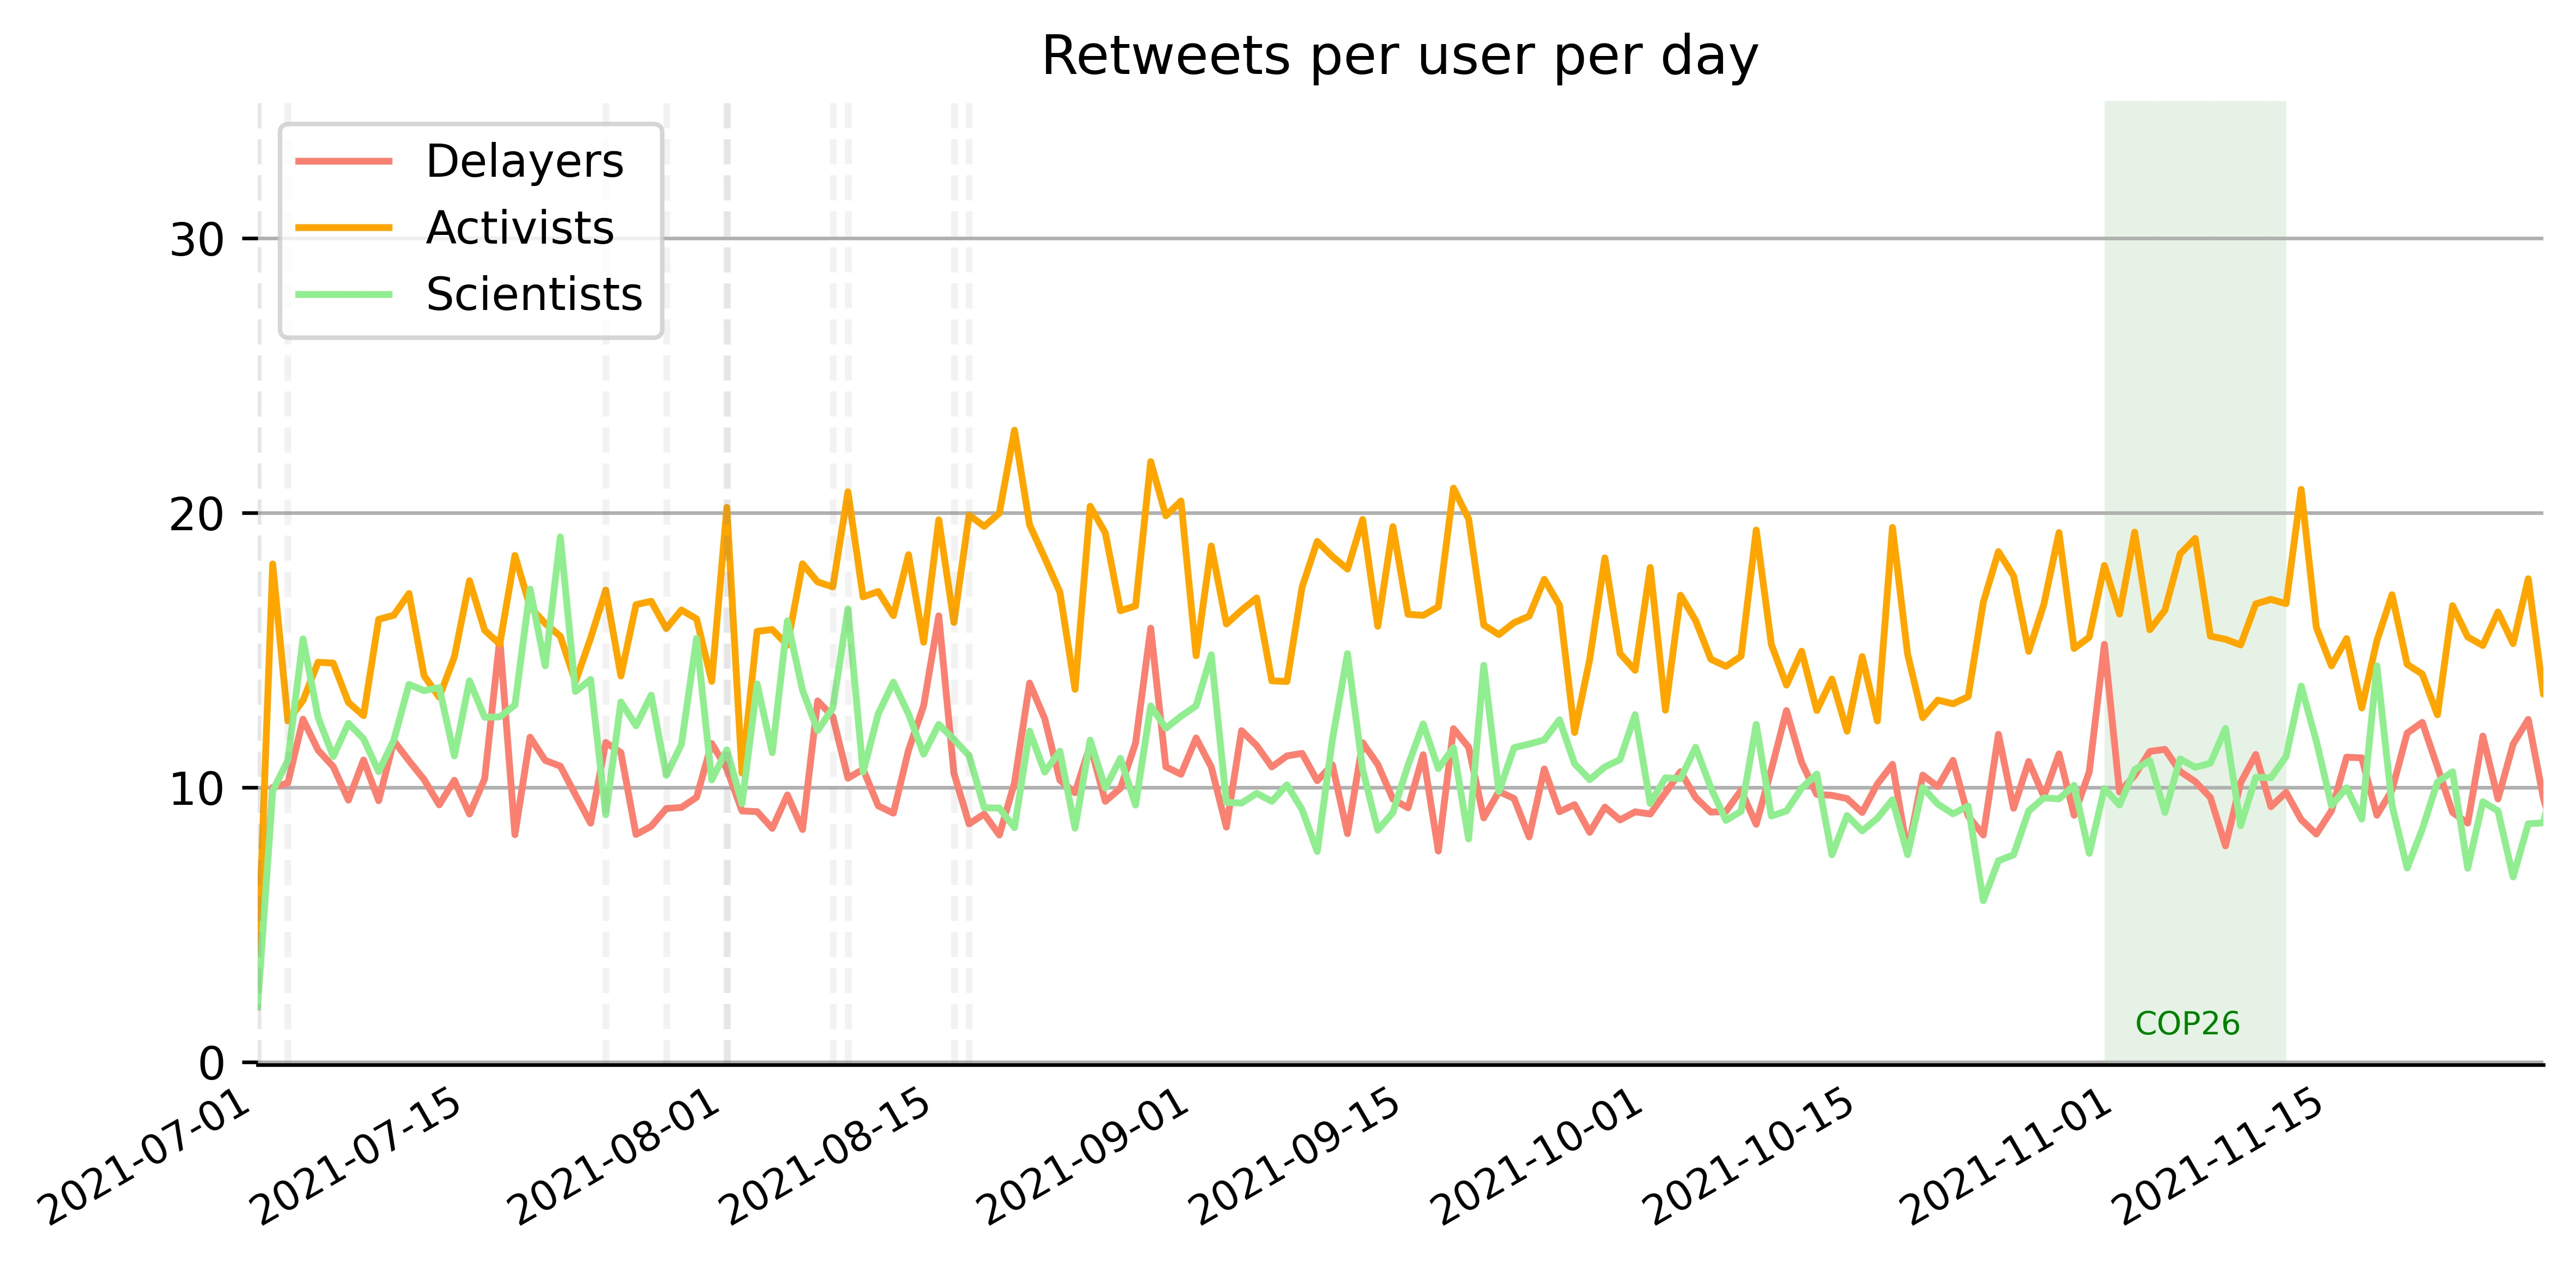
\includegraphics[width=.8\linewidth]{../figures/retweets_per_day_2022_07_28.jpg} 
    \caption{} 
  \end{minipage} 
  \begin{minipage}[b]{0.4\linewidth}
  \centering
    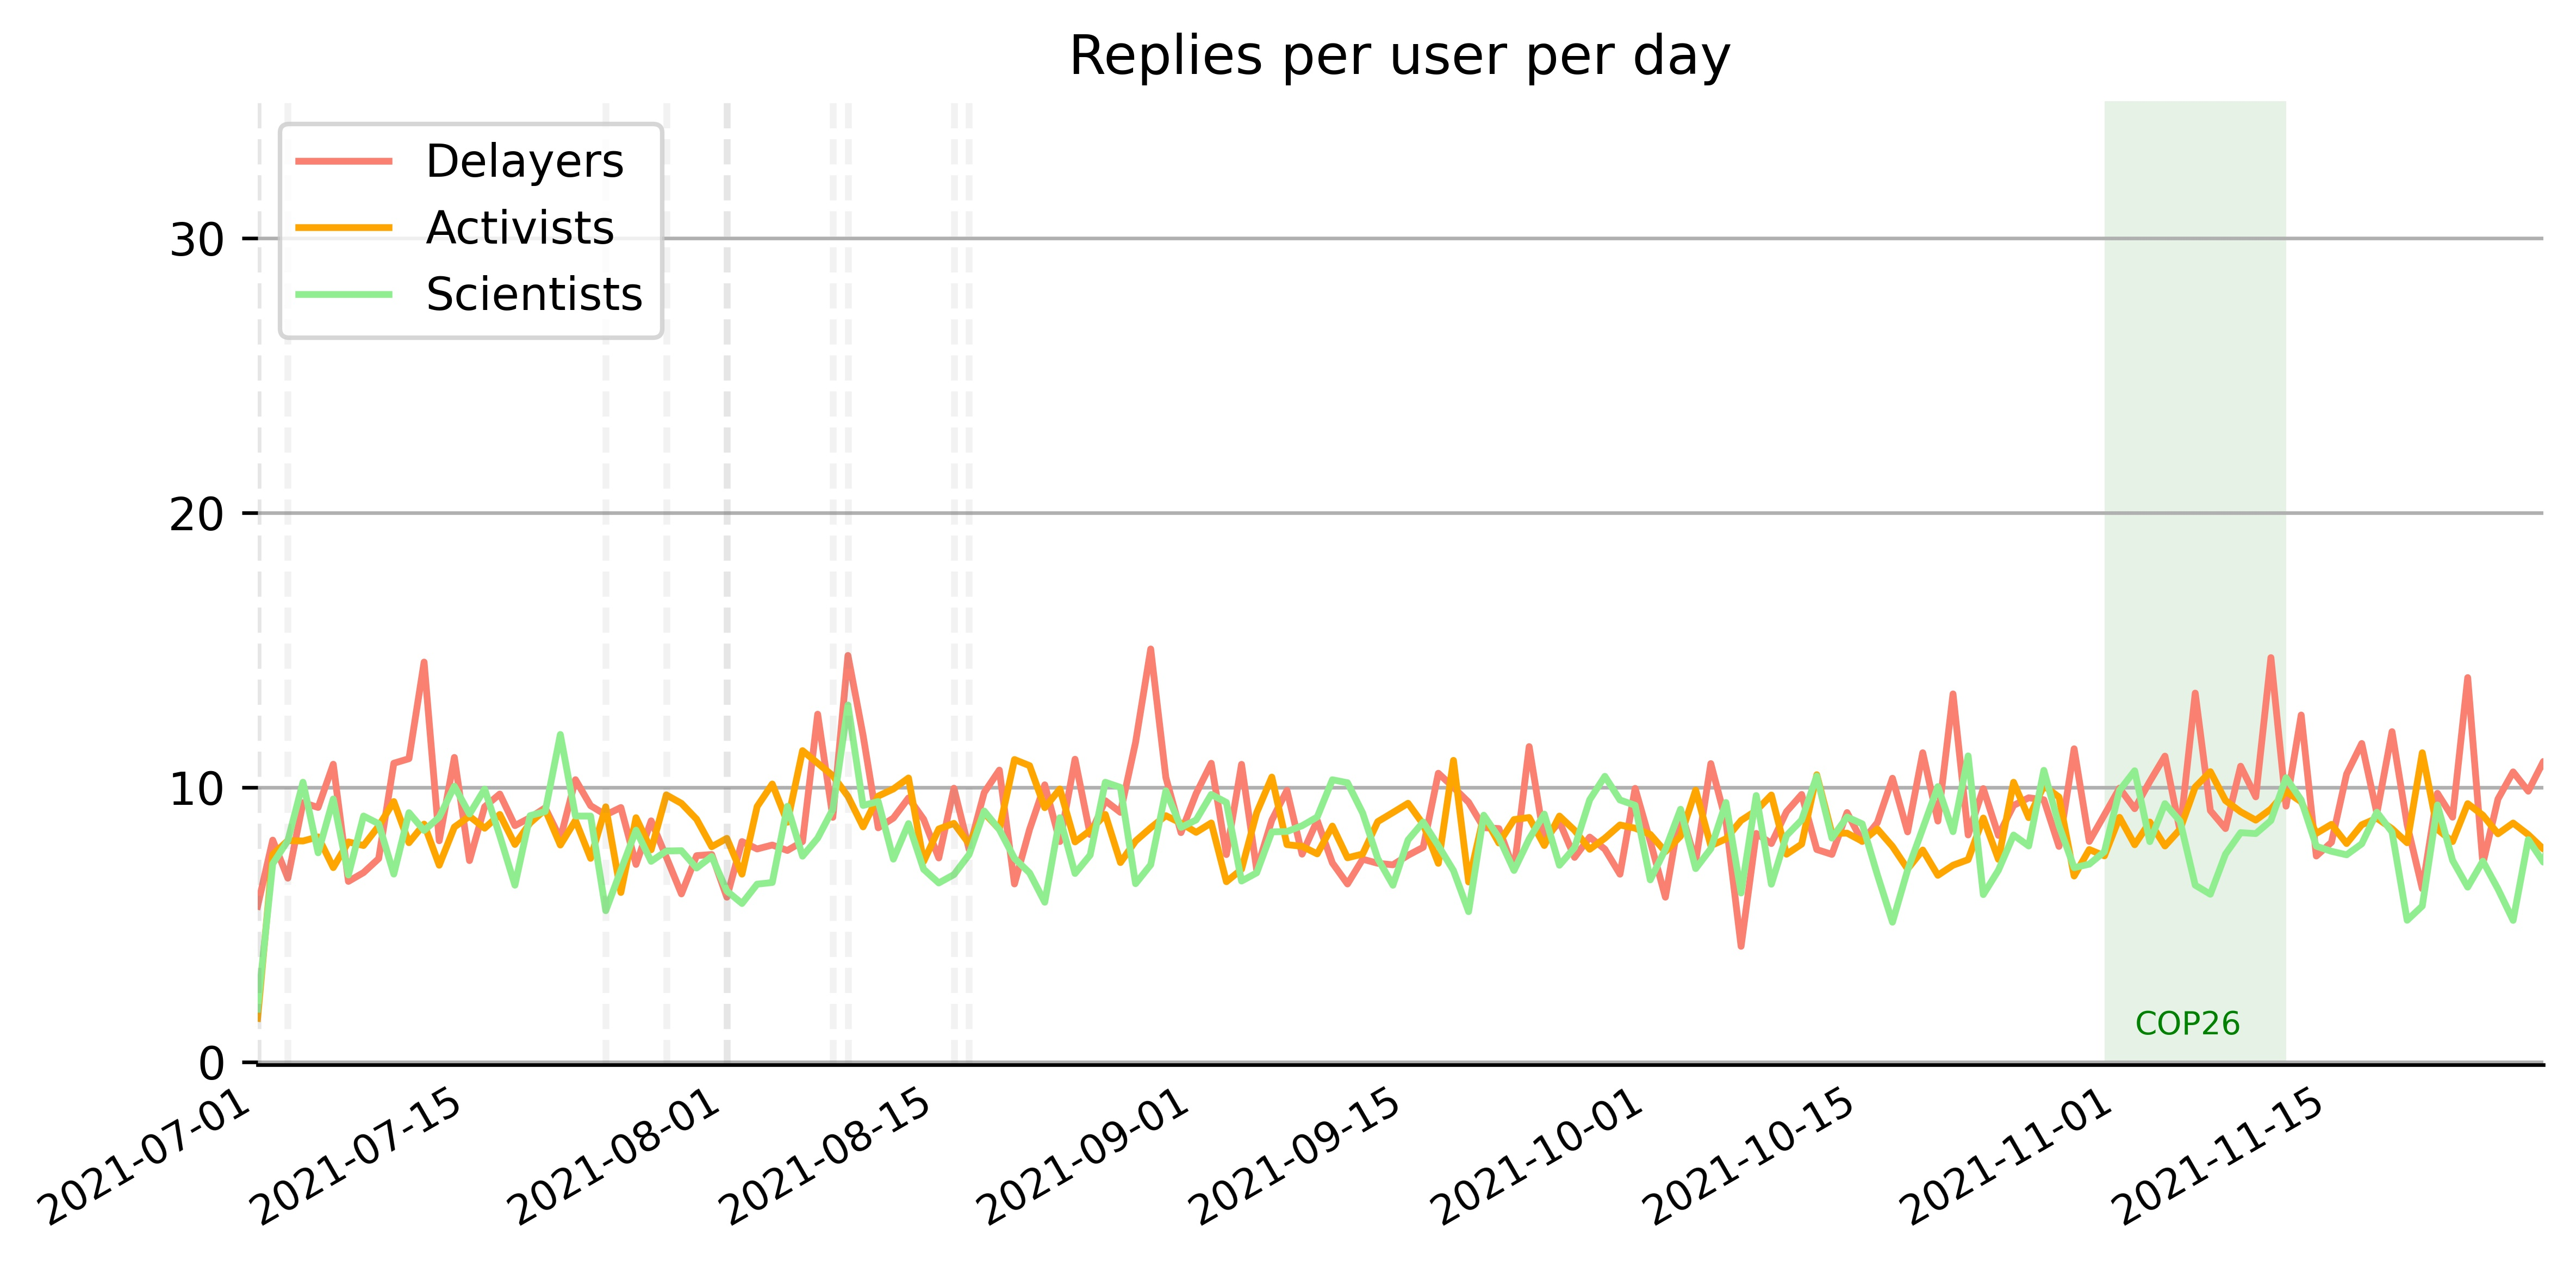
\includegraphics[width=.8\linewidth]{../figures/replies_per_day_2022_07_28.jpg} 
    \caption{} 
  \end{minipage} 
  \begin{minipage}[b]{0.4\linewidth}
  \centering
    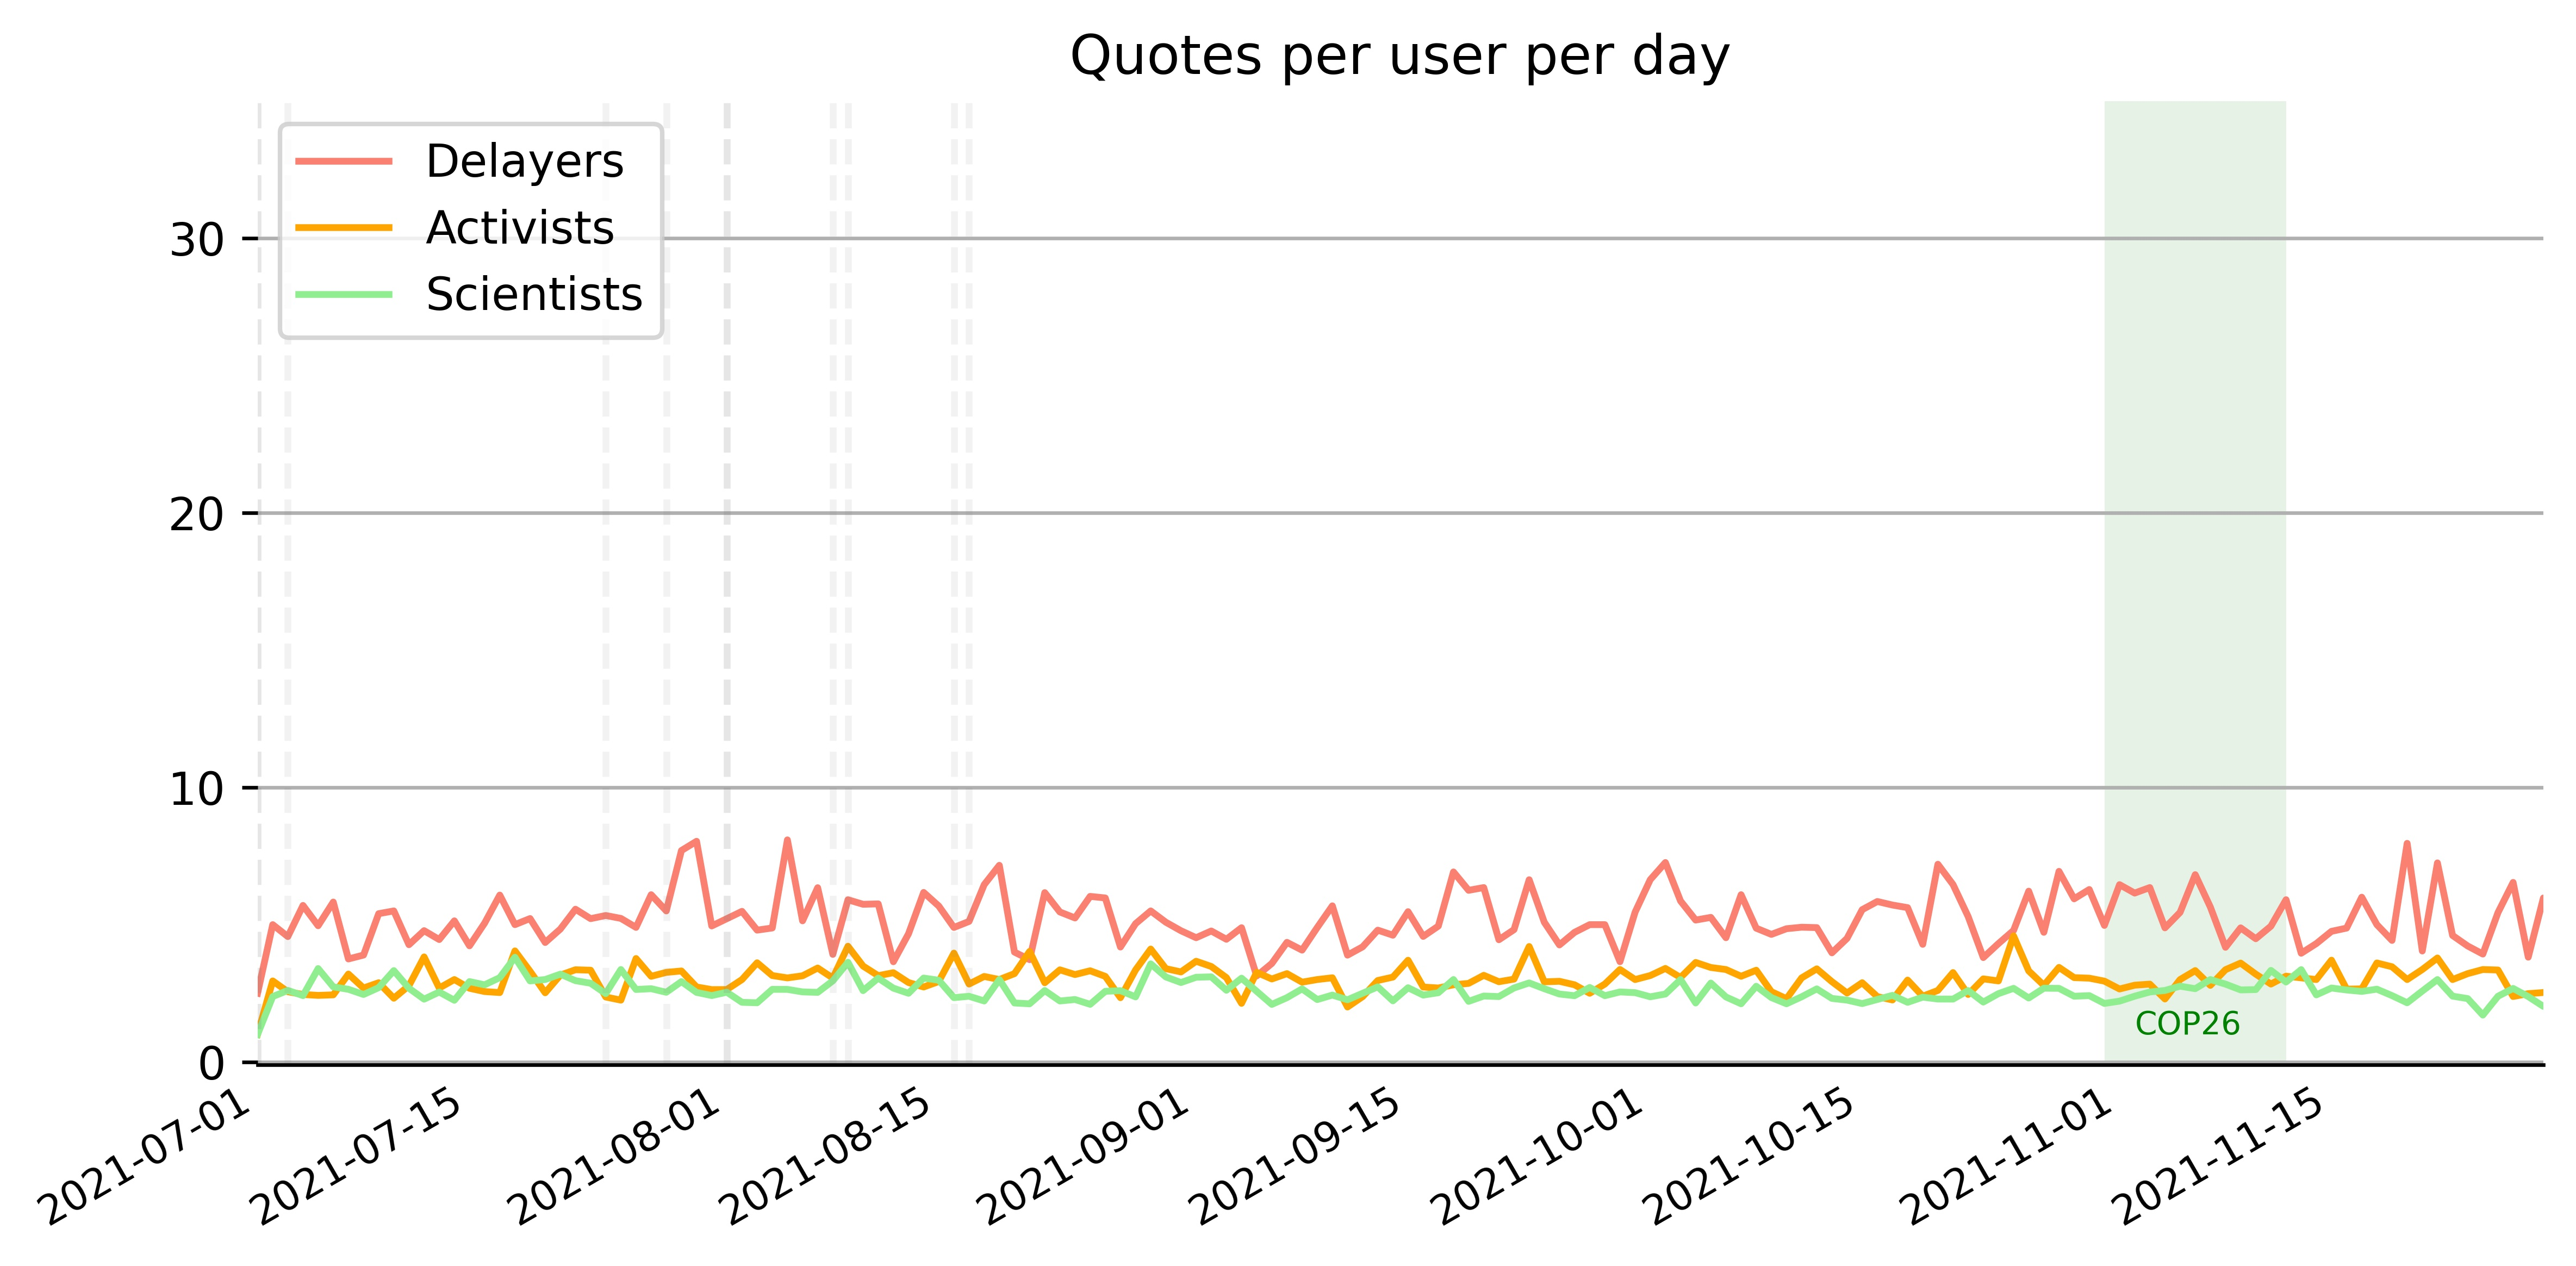
\includegraphics[width=.8\linewidth]{../figures/quotes_per_day_2022_07_28.jpg} 
    \caption{} 
  \end{minipage}
  \hfill
  \hfill
  \begin{minipage}[b]{0.4\linewidth}
  \centering
    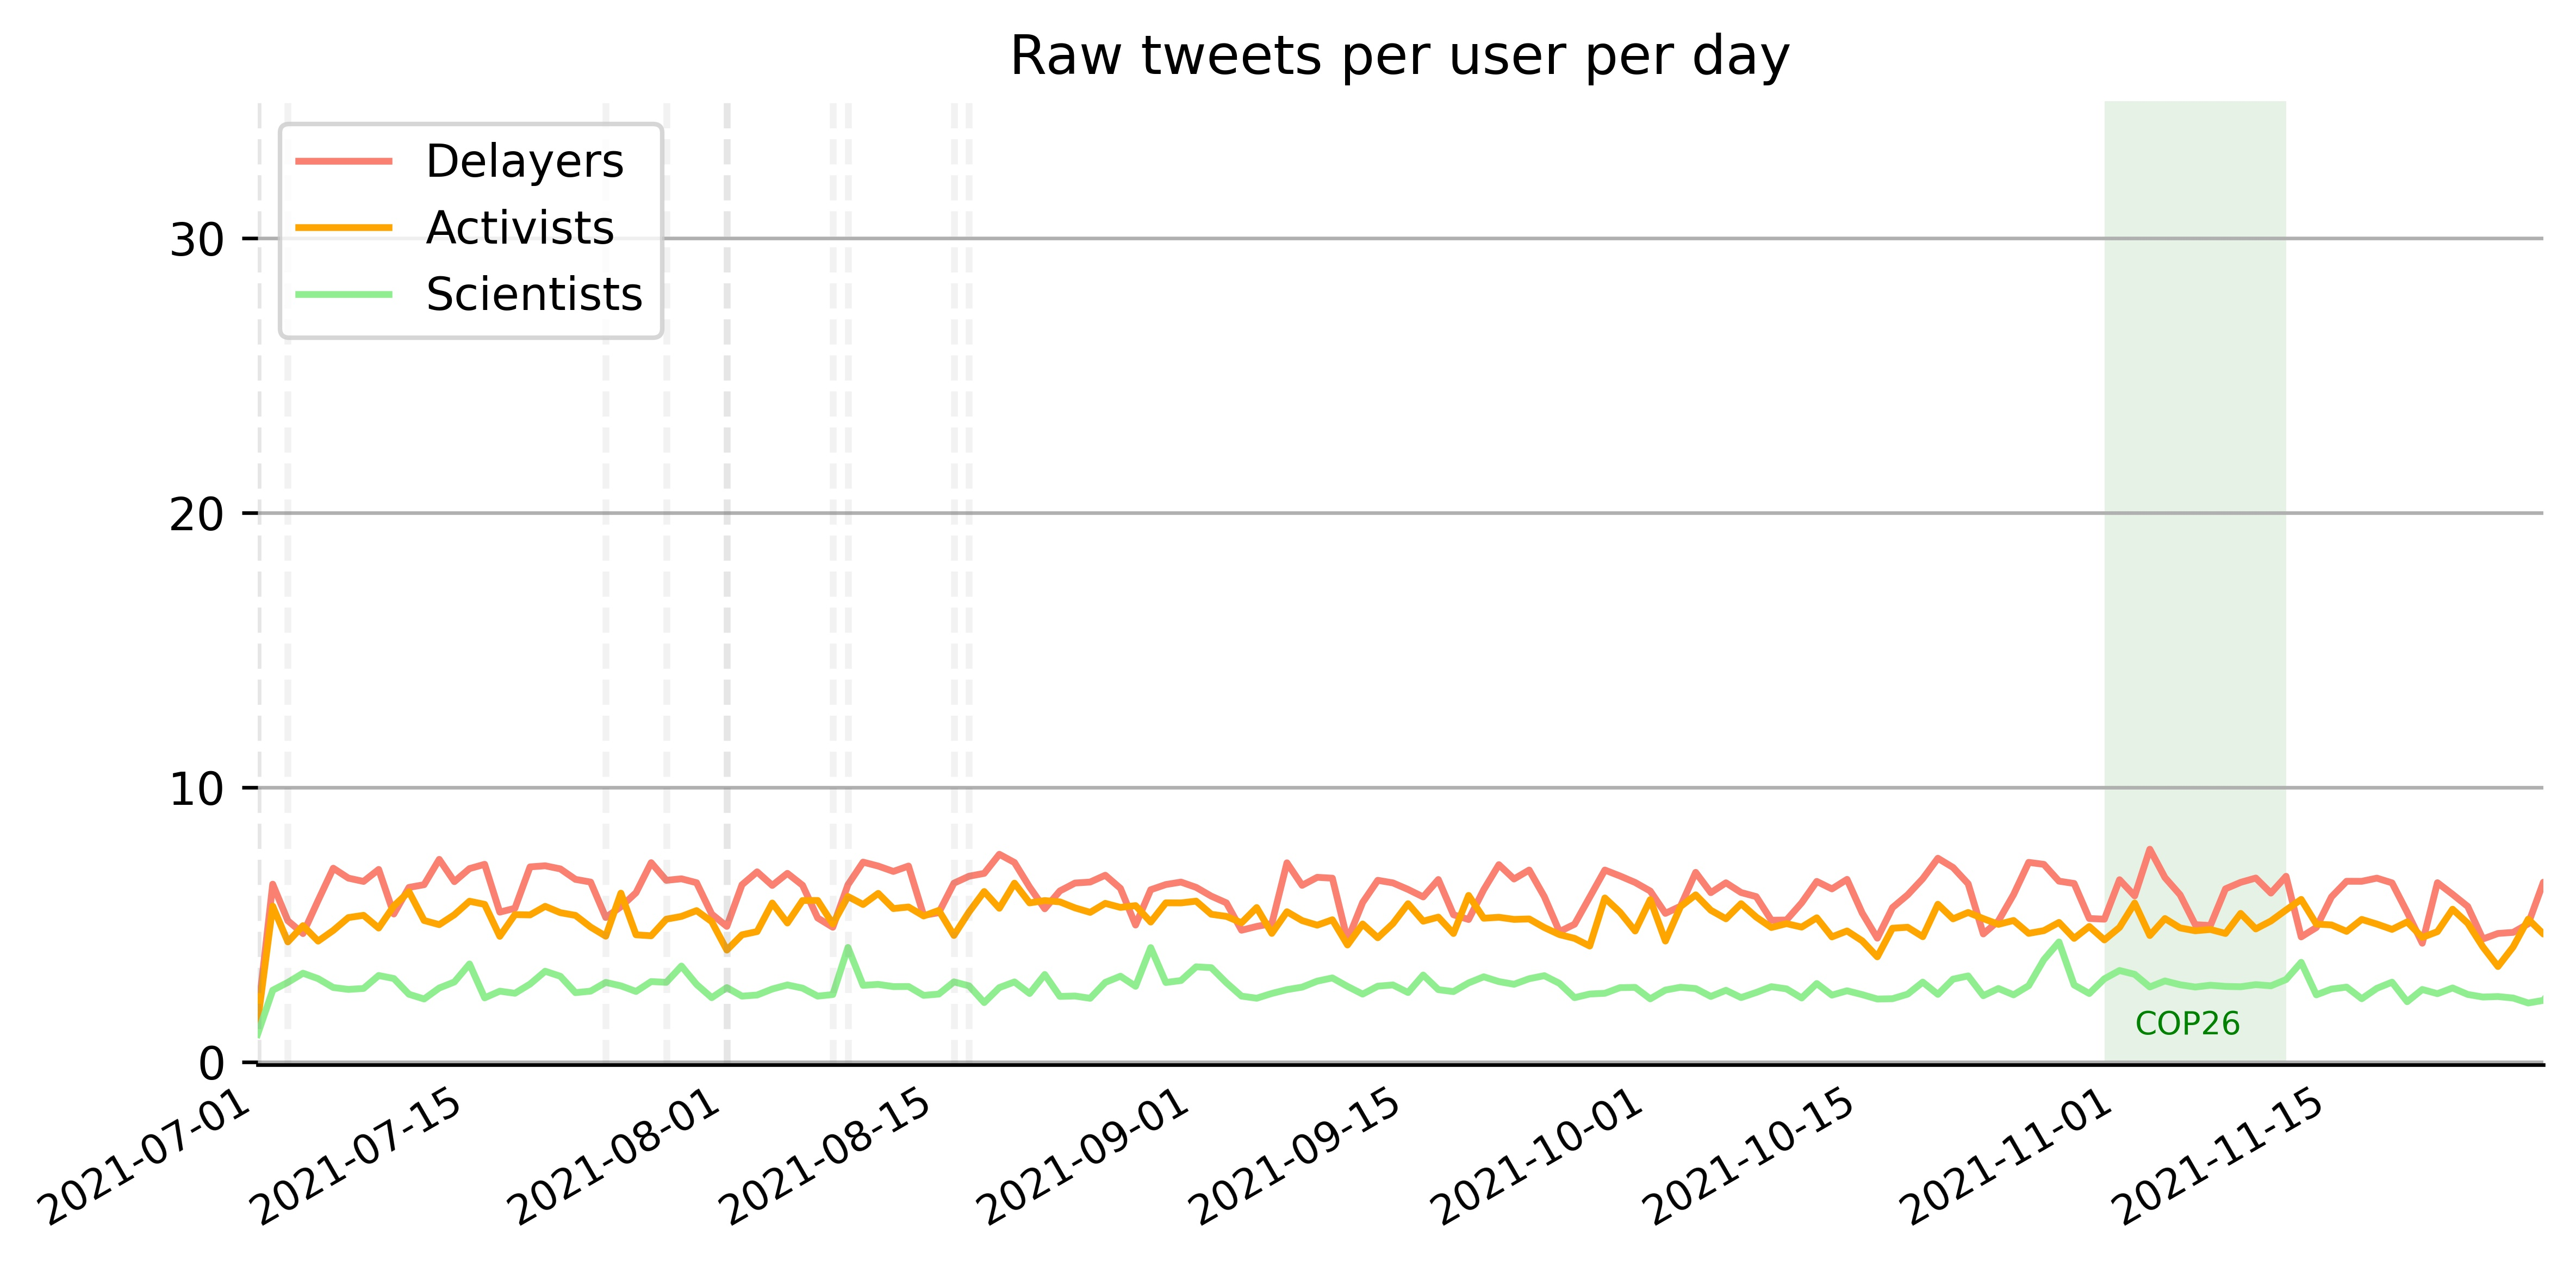
\includegraphics[width=.8\linewidth]{../figures/cc_per_day_2022_07_28.jpg} 
    \caption{} 
  \end{minipage} 
\end{figure}

\begin{figure}[ht] \label{ fig7} 
  \begin{minipage}[b]{0.3\linewidth}
  \centering
    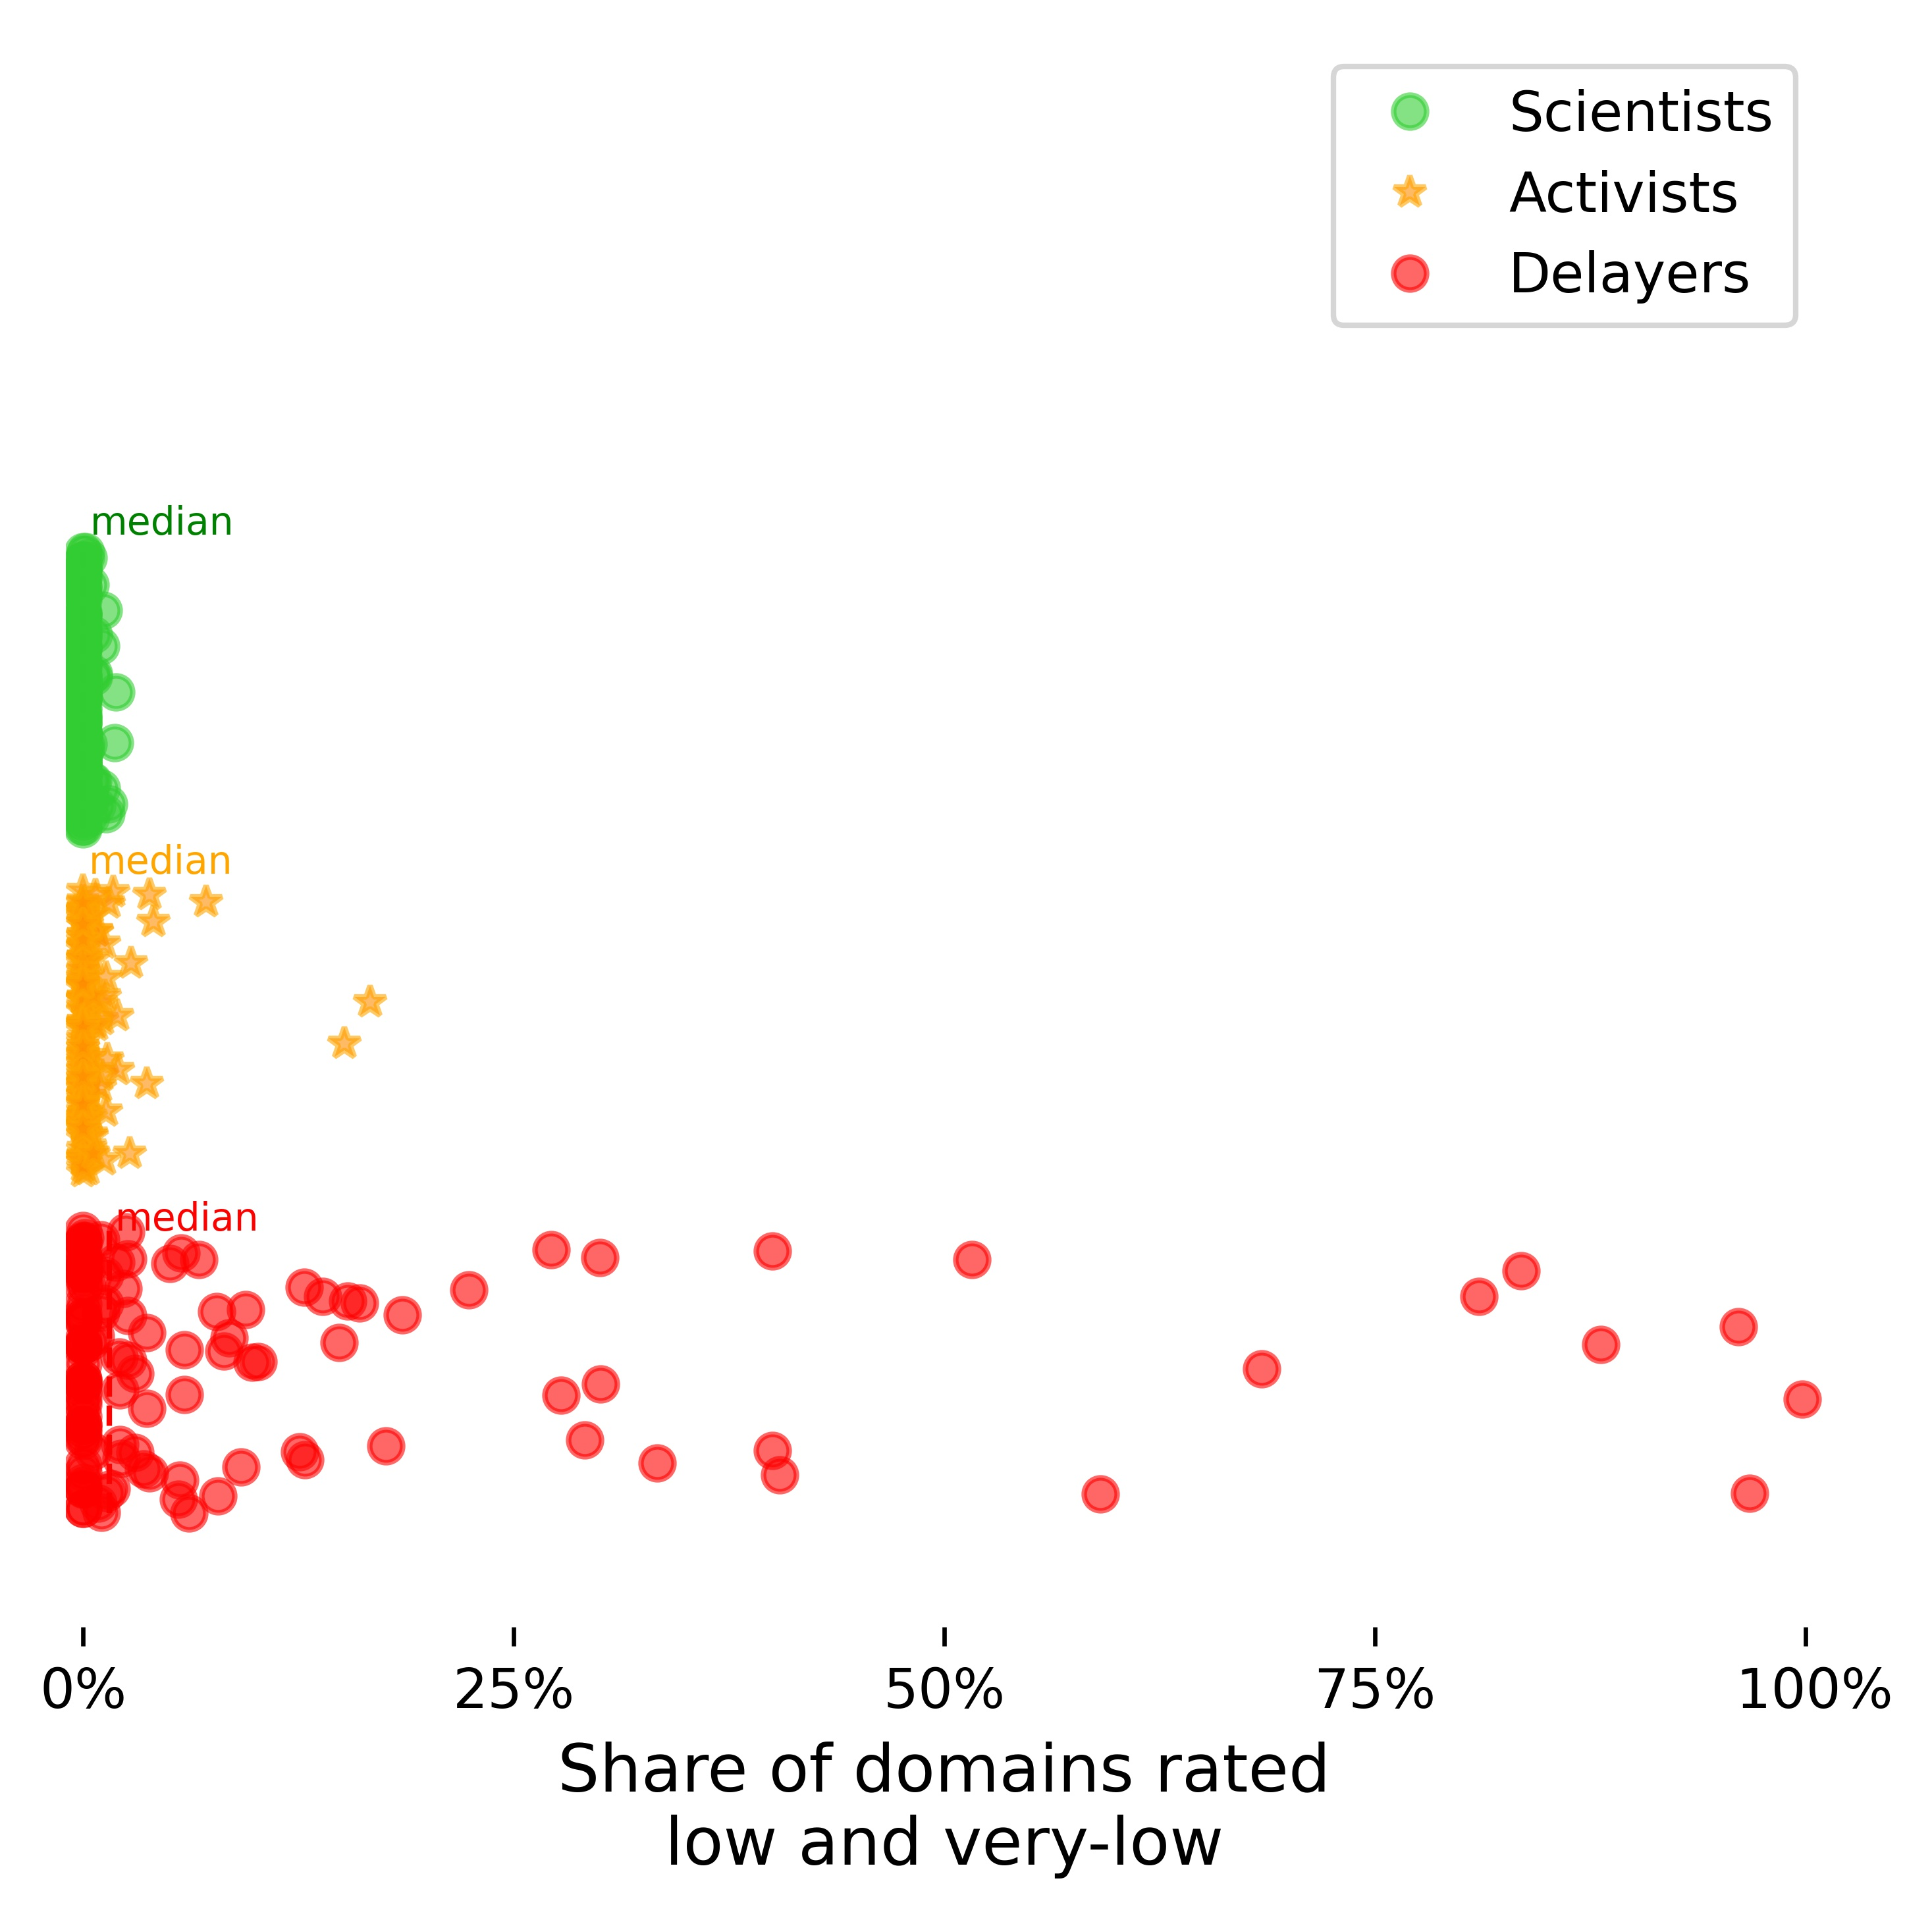
\includegraphics[width=.8\linewidth]{../figures/negative_rating_climate_agg_2022_07_29.jpg} 
    \caption{} 
  \end{minipage} 
  \begin{minipage}[b]{0.3\linewidth}
  \centering
    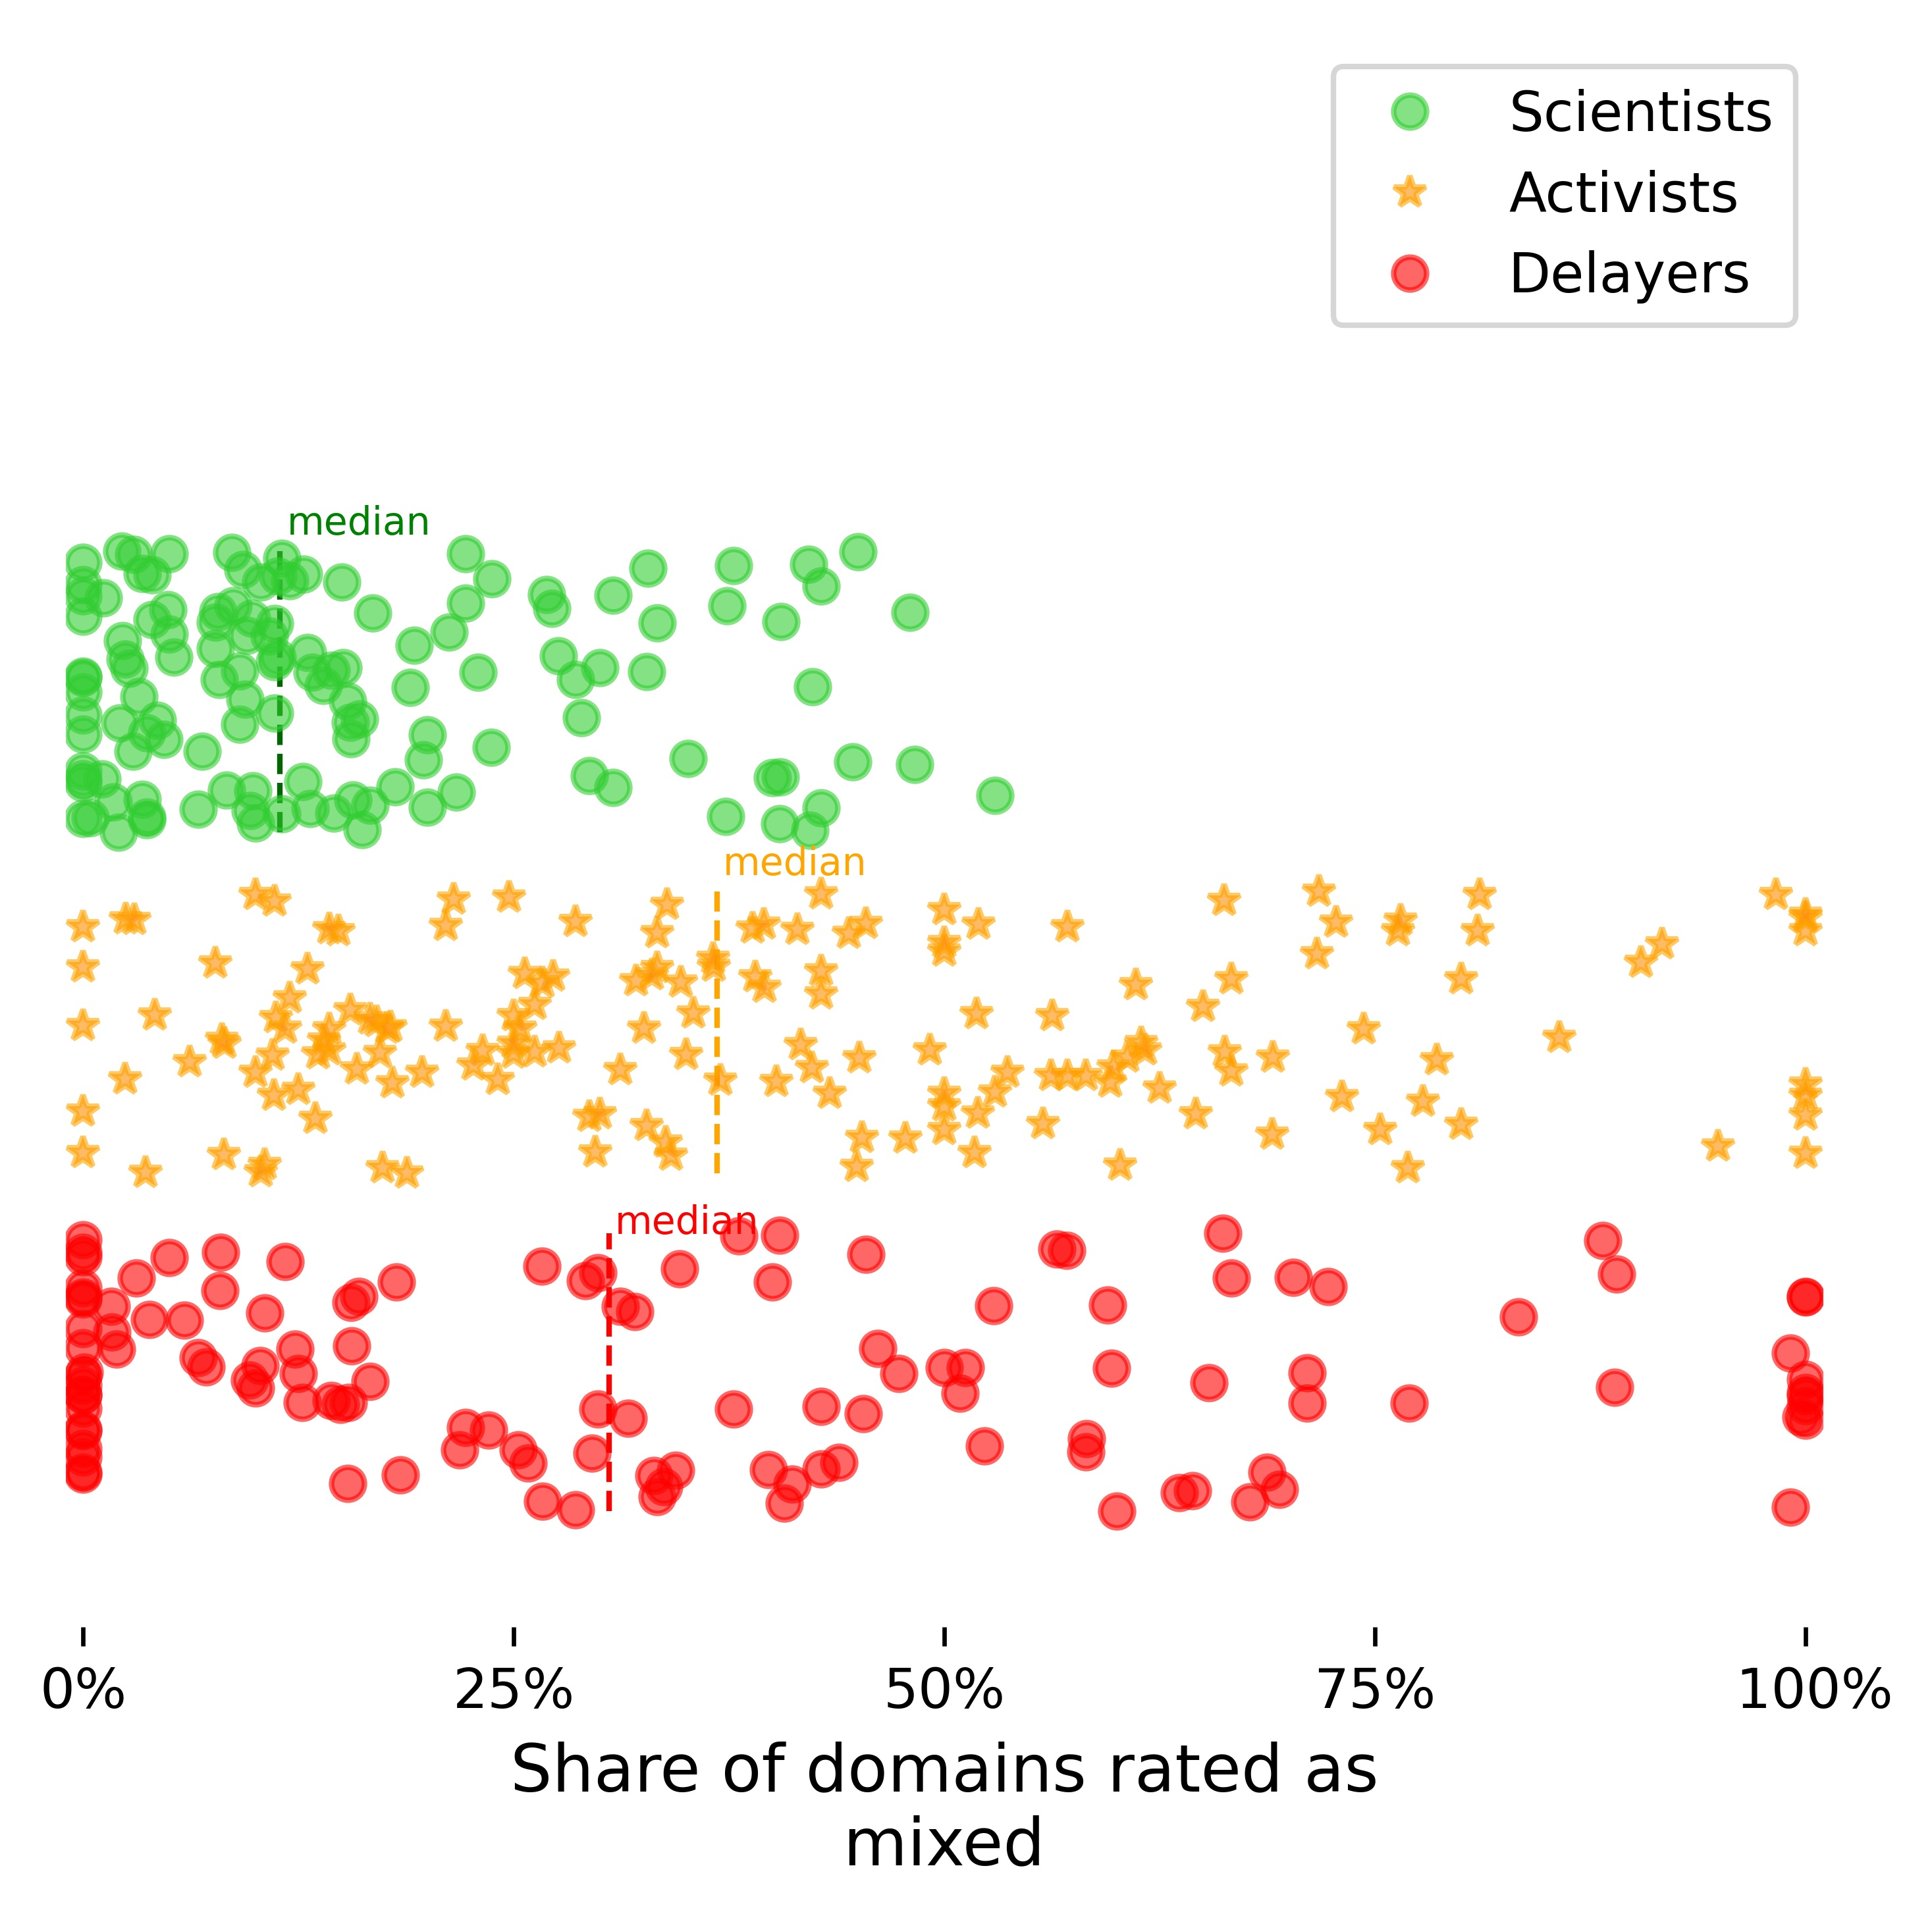
\includegraphics[width=.8\linewidth]{../figures/mix_rating_climate_agg_2022_07_29.jpg} 
    \caption{} 
  \end{minipage} 
  \begin{minipage}[b]{0.3\linewidth}
  \centering
    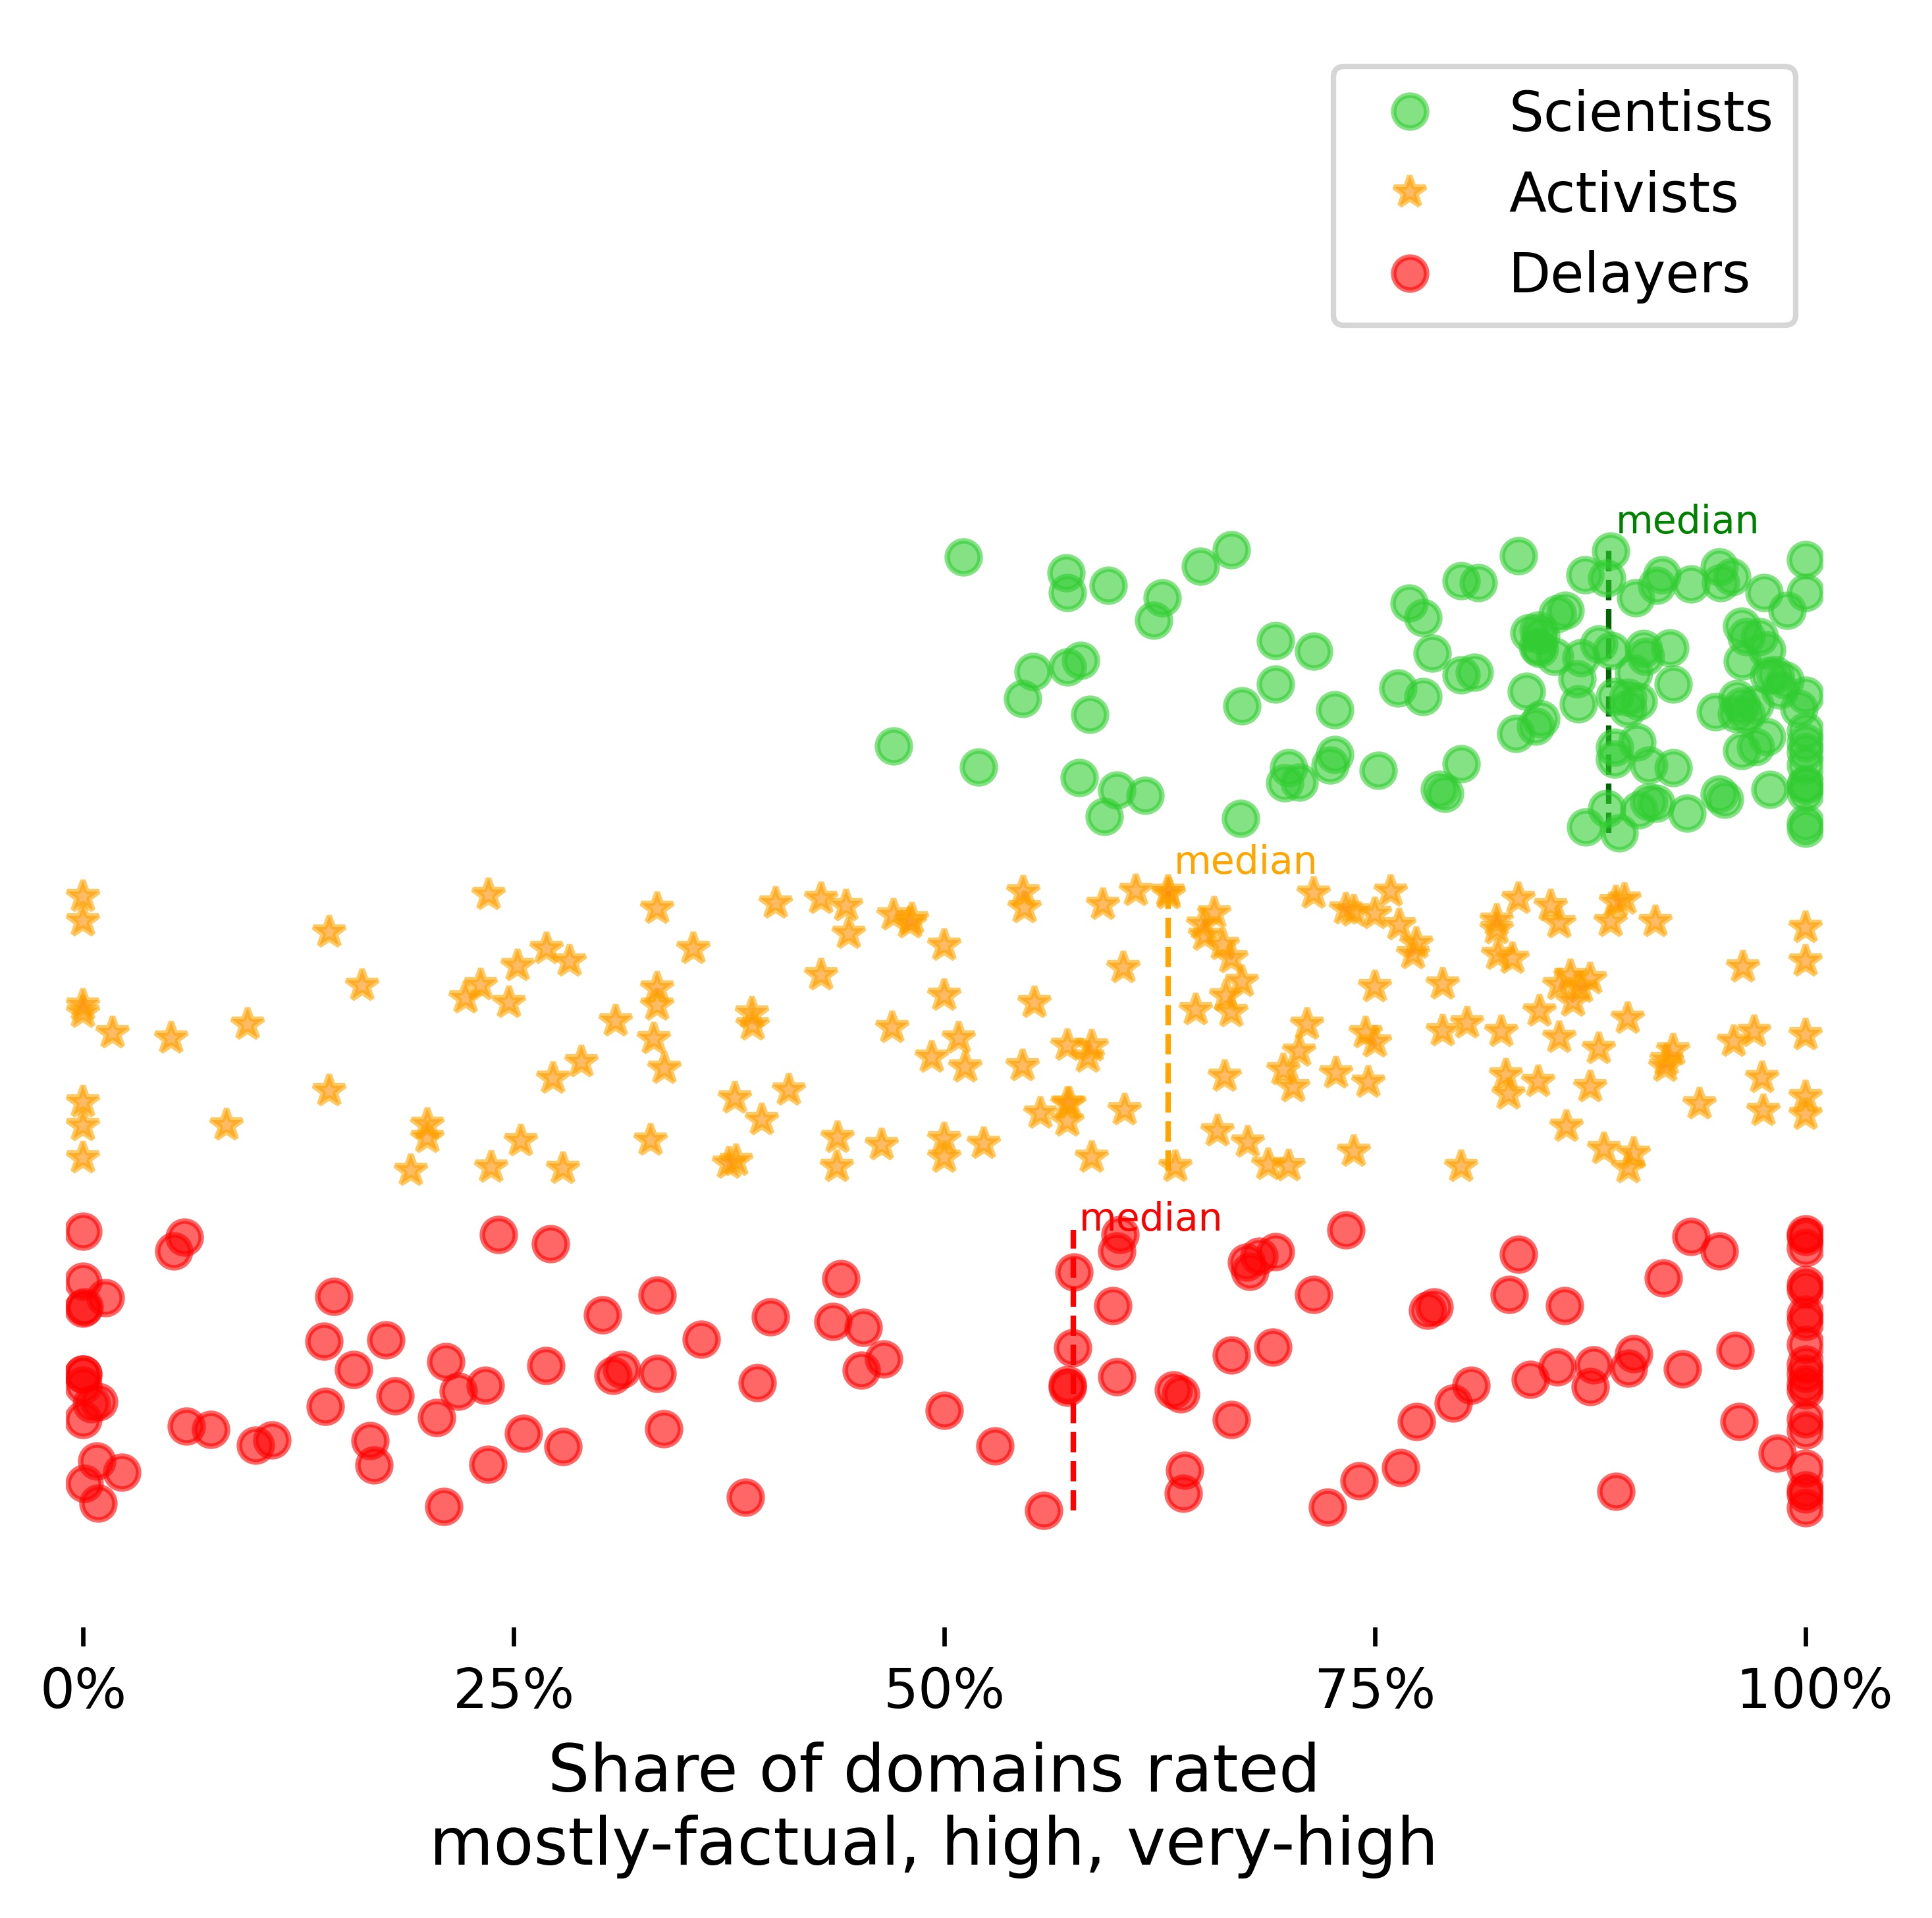
\includegraphics[width=.8\linewidth]{../figures/positive_rating_climate_agg_2022_07_29.jpg} 
    \caption{} 
  \end{minipage}
\end{figure}

\bibliography{res_statement}{}
\bibliographystyle{plain}

\end{document}